\section{Point spread function}
\label{sec:PSF}

In this section, we examine the point spread function (PSF) by studying a 3D stack of photos of beads that are
embedded in an agarose matrix. The matrix prevents the beads from moving. Since the beads are smaller
than the resolution, we can observe diffraction patterns. The diffraction pattern commonly observed for a spherical object is represented by an Airy function, which can be seen in \cref{fig:Airy}. 
Since the resolution is not sufficient to distinguish the secondary peaks from the main peak, they appear as shoulders.
\begin{figure}[h]
    \centering
    \begin{subfigure}{0.51\linewidth}
        \centering
        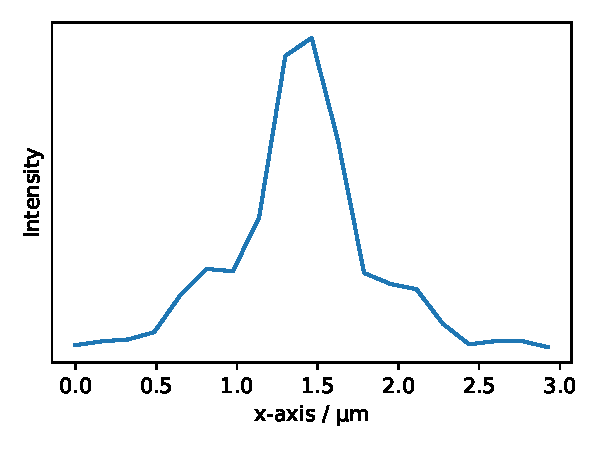
\includegraphics[width = \textwidth]{Bilder/PSF/Airy.pdf}
        \caption{Cut through the picture in \ref*{subfig:AiryBild}}
        \label{subfig:Airy}
    \end{subfigure}
    \hfill
    \begin{subfigure}{0.43\linewidth}
        \centering
        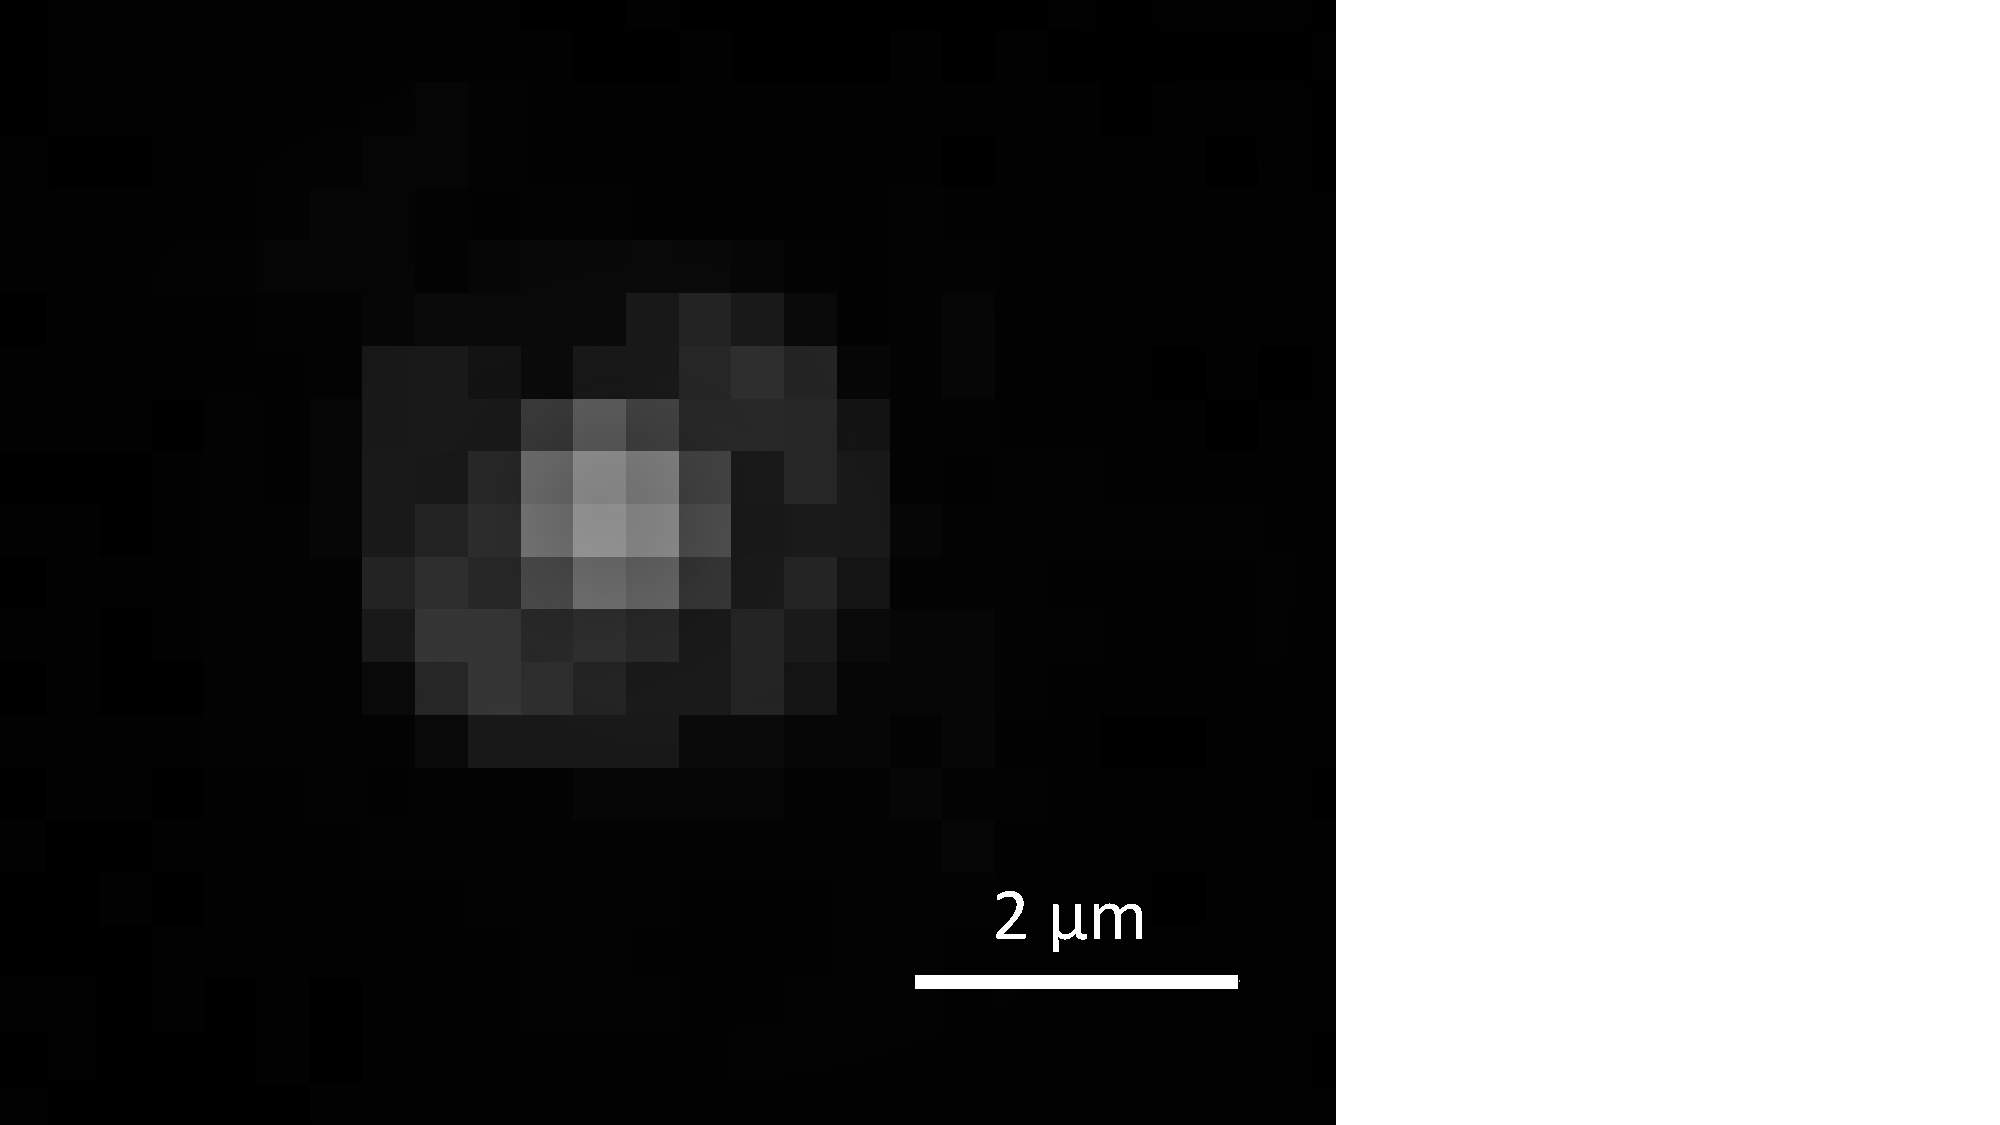
\includegraphics[width = \textwidth]{Bilder/PSF/2DBeugung_cropped.pdf}
        \caption{Image of a beat}
        \label{subfig:AiryBild}
    \end{subfigure}
    \caption{Image of a beat collected with a light sheet microscope (right) and a horizontal cut depicting the intensity profile (left). The intensity profile has one main peak and two separate smaller peaks, which appear as shoulders.}
    \label{fig:Airy}
\end{figure}


The particles were captured at four distinct locations (see \cref{fig:sites}) using no pinhole. Additionally, position 1 was imaged using both a half-open and a closed pinhole. Notably, the particles at positions 2 and 3 exhibited significant aberrations (see \cref{tab:FWHM}).
Conversely, the particles at positions 4 and 1 displayed small aberrations, which led to the selection of position 1 for subsequent measurements.


The FWHM is extracted using a Gaussian fit to the cuts, as shown in \cref{subfig:Airy}. The fitting is
performed using \textit{scipy.optimize.curve\_fit()}. Since the amount of available data does not allow
for its calculation, the uncertainty is not estimated. For each case, three beads in and out of
focus are analyzed. The results are presented in \cref{tab:FWHM}.

We encountered challenges in certain cases when identify to locate out-of-focus beads as there is no clear criteria to distinguish the two species.
Additionally, we experienced issues with the data from position 2. Our initial attempt to measure the stack of images was unsuccessful. 
Upon restarting the measurement, no beads were visible anymore. The images captured prior to the measurement failure depict heavily distorted beads, making them unsuitable for analysis using Gaussian fits.
Our reconstruction of the situation leads us to believe that we made the sample crash into the objective lens. This changes the optical properties of the objective lens because 
the refractive index difference is different. The force on the objective lens causes the programme to crash. Due to the impact, the sample was shifted out of focus. Therefore in the second measurement nothing is to be seen.
Furthermore, some interesting effects appear in the data. Certain patterns can be observed from time to time in our data. We do see for example 
some kind of smudged images as shown in \cref{fig:Verueckttebeats}. This look like the motor was from time to time not synchronized with the clock of the motor. 

\begin{table}[ht]
    \centering
    \begin{tabular}{cccc}
        \toprule Position 1: FWHM / $\SI{}{\micro \meter}$ & \textbf{x} &\textbf{y} & \textbf{z} \\
        \hline\hline open pinhole & $0.82\pm0.04$ & $0.84\pm0.04$ &  $3.1\pm0.4$ \\
        & \textcolor{gray}{$0.90\pm0.03$} & \textcolor{gray}{$1.06+0.03$} & \textcolor{gray}{$3.3+0.1$}\\
        half open pinhole & $1.00 \pm0.04$ &$ 0.86\pm0.06 $& $2.6\pm0.6$ \\
        closed pinhole & $0.60 \pm 0.09$ & $0.59 \pm 0.06$ & $2.6\pm0.6$ \\
        % \hline Position 2:  & & &  \\
        % \hline open pinhole & $0.82\pm0.04$ & $0.84\pm0.04$ & $add$ \\
        %  & \textcolor{gray}{$0.90\pm0.03$} & \textcolor{gray}{$1.06\pm0.03$} & \\
        \hline Position 3: FWHM / $\SI{}{\micro \meter}$  & & &  \\
        \hline open pinhole & $0.76\pm0.04$ & $ 1.18\pm0.02$ & $7.9\pm0.8$ \\
        & \textcolor{gray}{$0.73\pm0.01$} & \textcolor{gray}{$1.03\pm0.05$} & \textcolor{gray}{$7.2\pm0.9$}\\
        \hline Position 4: FWHM / $\mathrm{mm}$  & & &  \\
        \hline open pinhole & $0.67\pm0.01$ & $0.54 \pm 0.02$ & $4.5\pm 0.8$ \\
        & \textcolor{gray}{$1.03\pm0.03$} & \textcolor{gray}{$0.78+0.02$} & \textcolor{gray}{$9.5+0.9$}\\
        \bottomrule
    \end{tabular}
    \caption{FWHM of the PSF fitted from cuts through 2D arrays of intensity. }
    \label{tab:FWHM}
\end{table}

The data collected indicate that closing the pinhole results in a narrower PSF. Thats is what we expected as closing the pinhole narrows down the light sheet. This should be especially visible in the z-component. This trend can be observed in the data, but the errors are to big to call the effect significant. 
We also observe a tendency for the beads out of focus to have a broader FWHM. This is also to be expected, as the 
process of being out of focus distorted the actual peak. As deciding which beat is out of focus is a 
subjective decision which depends among other aspects on the broadening of the peak, this result is not very surprising.
So the observation might also just indicate a tendency to categorize broader peaks as "out of focus" due to subjective preferences.

The anisotropy in the x- and y-directions at positions 3 and 4 can be explained by symmetry break due to the positioning of the surface liquid. This observation is consistent with position 1, which shows equal FWHM in both directions. The lower resolution in the z-direction is attributed to the larger motor steps. Furthermore, there is a systematic error in the analysis as fitting in the z-direction is not feasible due to the movement (or jiggling) of the beads. As a result, the estimation of the z-component relies on the number of images where the object is visible. Additionally, the extraction of the Point Spread Function (PSF) in the z-direction assumes the presence of a true 2D light sheet, which is not accurate as shown in \cref{sec:LightSheet}.